%% Figure: PSP E4 Alfvenic control -- CD vs gradient fire rates by window class
%% Data source: data/output/heliosphere/ablations/psp_alfven_control.json
%% Experiment: E-269  |  Claim: registration pending
%%
%% Window classes defined by +-5 min sliding classifier:
%%   Alfvenic:            Br sign reversal within +-5 min
%%   CompressiveBoundary: delta_B/|B| > 0.3 without sign reversal
%%   Quiet:               neither condition
%%
%% PSP Encounter 4: 2020-01-20 to 2020-02-10, perihelion 2020-01-29 ~27.9 Rs  (31673 minutes)
\documentclass[tikz,border=4pt]{standalone}
\usepackage{pgfplots}
\pgfplotsset{compat=1.18}
\usepackage{xcolor}

\definecolor{OIorange}{RGB}{230,159,0}
\definecolor{OIskyblue}{RGB}{86,180,233}
\definecolor{OIgray}{RGB}{153,153,153}

\begin{document}
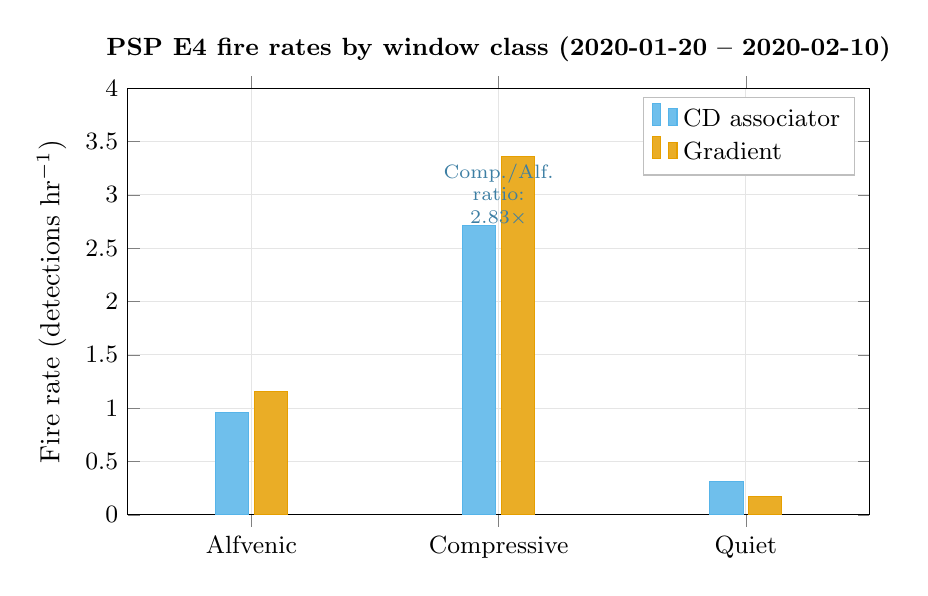
\begin{tikzpicture}
\begin{axis}[
    ybar,
    bar width=12pt,
    width=11cm,
    height=7cm,
    enlarge x limits=0.25,
    ylabel={Fire rate (detections hr$^{-1}$)},
    ymin=0, ymax=4.0,
    ytick={0,0.5,1.0,1.5,2.0,2.5,3.0,3.5,4.0},
    symbolic x coords={Alfvenic, Compressive, Quiet},
    xtick=data,
    xticklabel style={font=\small},
    yticklabel style={font=\small},
    legend style={at={(0.98,0.98)}, anchor=north east, font=\small,
                  draw=gray!50, fill=white},
    legend cell align=left,
    grid=major,
    grid style={gray!20},
    title style={font=\small\bfseries},
    title={PSP E4 fire rates by window class (2020-01-20 -- 2020-02-10)},
]

%% CD associator rate (detections/hr)
\addplot[fill=OIskyblue!85, draw=OIskyblue] coordinates {
    (Alfvenic,    0.958)
    (Compressive, 2.711)
    (Quiet,       0.311)
};
\addlegendentry{CD associator}

%% Gradient rate
\addplot[fill=OIorange!85, draw=OIorange] coordinates {
    (Alfvenic,    1.155)
    (Compressive, 3.360)
    (Quiet,       0.168)
};
\addlegendentry{Gradient}

%% Annotate discrimination ratio
\node[font=\scriptsize, align=center, text=OIskyblue!70!black] at
    (axis cs:Compressive, 3.0)
    {Comp./Alf.\\ratio:\\$2.83\times$};

\end{axis}
\end{tikzpicture}
\end{document}
